\chapter{Background information and theory}
\label{Chapter3}

\section{Abstract syntax tree}
The \emph{abstract syntax tree} is a tree representation of an abstract structure of programming code. For each expression or statement in the code, abstract syntax tree assigns the corresponding node. Abstract syntax tree could not contain all the details of the underlying code like parentheses or indentation, but its structure allows to interpret a code execution process unambiguously. The established grammar of abstract syntax tree reduces search space of the model and implies the validity of generated code.

\begin{figure}[h]
\centering
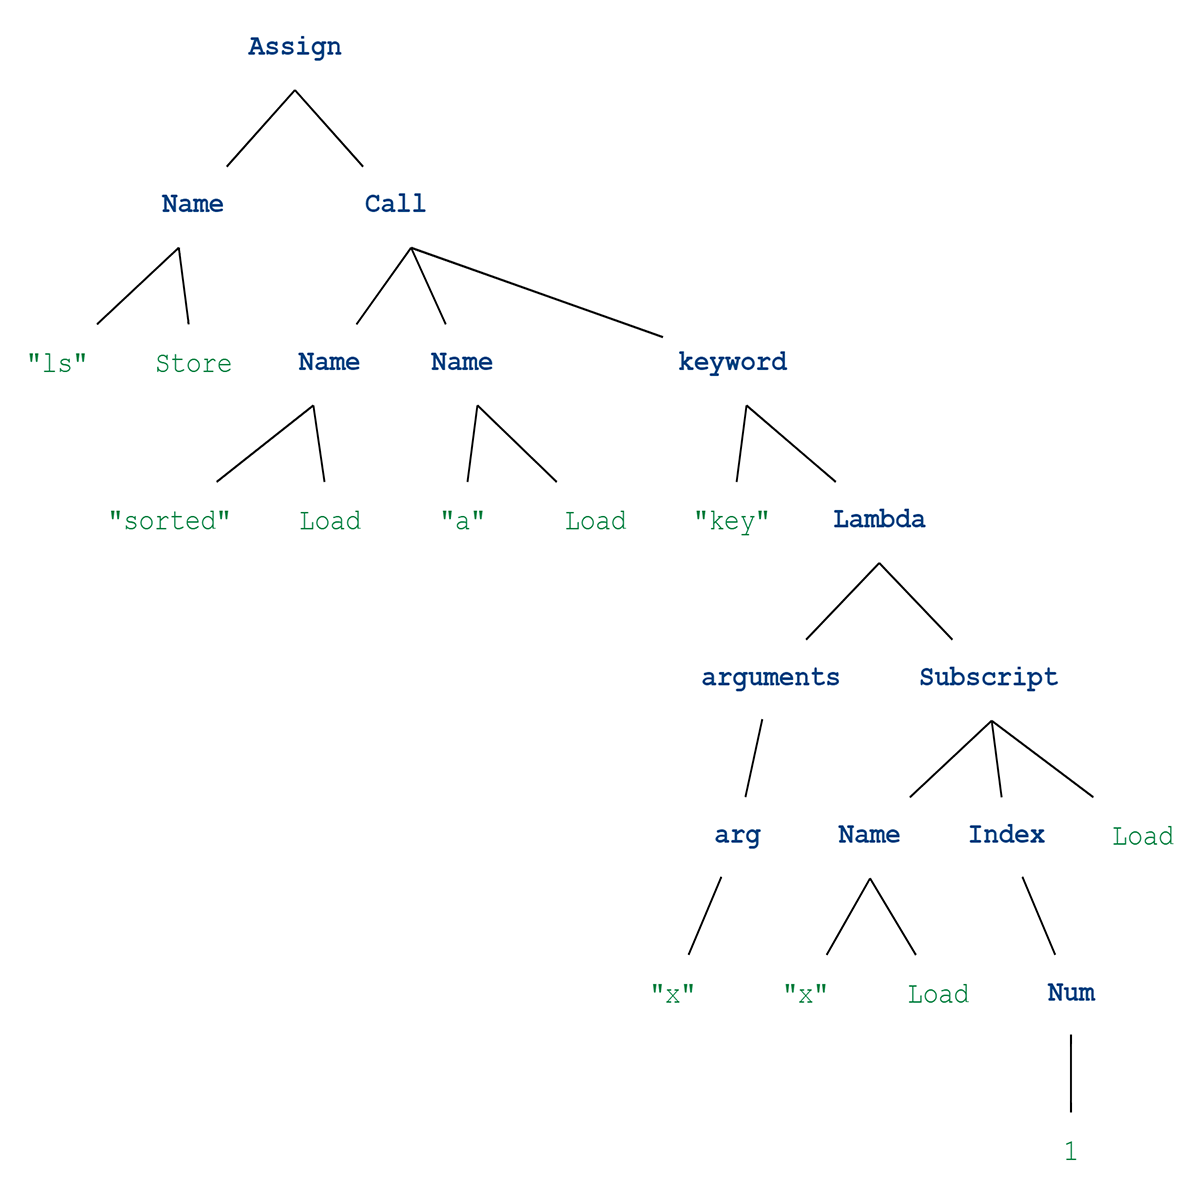
\includegraphics[width=5in]{Figures/ast}
\decoRule
\caption[Abstract Syntax Tree]{Abstract syntax tree of code snippet \code{ls = sorted(a, key=lambda x: x[1])}\protect\footnotemark.}
\label{fig:ast}
\end{figure}

\footnotetext{Picture is created in Python library \href{https://github.com/hchasestevens/show_ast}{showast}.}

The Python \emph{abstract grammar} contains a set of production rules, composed of head node and multiple child nodes. For example, in \cref{fig:ast} the first rule is used to generate the assignment of statement result to variable. It consists of the head node of type \code{Assign} and two child nodes of types \code{Name} and \code{Call}, respectively. Non-terminal nodes (the blue ones) defines the  structure of the target code, while terminal nodes (the green ones) refer to symbol tokens, like variables, constants or operations. Full Python 3.6 abstract grammar can be found in  \cref{AppendixA}. 

\section{syntactic parsing}
\subsection{Constituency parsing}
Theory of sentence analysis is derived from the idea that the words of a sentence seem to combine into patterns and structures. Each word is classified as a different in terms of its function in a sentence. According to this function, to each word there can be assigned its lexical category or part of speech, like a noun (\code{N}), adjective (\code{A}), or verb (\code{V}). 

This system could be extended to the level of syntactic categories, combining words or other syntactic categories with similar function into phrases. Each phrase is characterized by the properties of the headword that it includes. For example, the headword of the subject of a sentence is a noun, so it is classified as a noun phrase (\code{NP}). A verb is regarded as the head of the sentence predicate, so predicate is classified as a verb phrase (\code{VP}). Rules which describe how lexical categories can be combined into syntactic categories is called \emph{rewriting rules}. For example, a noun phrase category may be described as the parent of adjective and noun categories, and it may be represented by a rule of the following form:

\begin{verbatim}
NP => A N
\end{verbatim}

A formalization of such rule-based sentence structure system is called a \emph{phrase-based grammar} or \emph{constituency grammar}. Grammar is defined by the following constituents:
$V_N$ is a non terminal vocabulary, which contains the lexical and syntactic category labels;
$V_T$ is terminal vocabulary and it contains a set of words.
$P$ identifies the collection of the production rules of the grammar.
To illustrate this concept, we present a short grammar to parse a sentence \textquote{good dogs like cats} to its syntactic representation. The grammar for this example contains the following vocabulary:
\begin{equation}
\begin{split}
V_N = {S, NP, VP, A, N, V}\\
V_T = {cats, dogs, like, good}
\end{split}
\end{equation}
The production rules for this grammar would be following:
\begin{verbatim}
S => NP VP
NP => A N
NP => N
VP => V NP
N => dogs
N => cats
V => like
A => good
\end{verbatim}
Graphic representation of syntactic tree  of this sentence can be seen in \cref{fig:syntax_tree}.

Phrase-based grammar might also be referred as a \emph{context-free grammar}, because it provides mechanism for combining a phrases from their constituents without usage of sentence context.

\begin{figure}
\centering
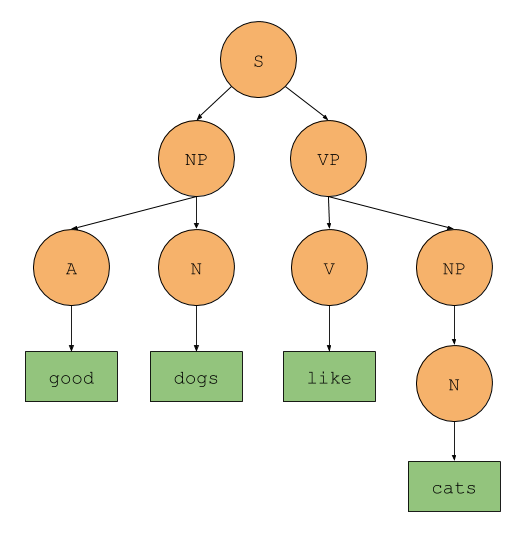
\includegraphics{Figures/syntaxtree}
\decoRule
\caption[Syntax tree]{Example of syntax tree.}
\label{fig:syntax_tree}
\end{figure}

\subsection{Combinatory-categorial grammar}
Phrase-structure grammars analyze the sentence recursively applying rewriting rules, starting from identification of the parts of speech or lexical categories of individual words. This rule governs how words can be combined into phrases and sentences. Compared with phrase-structure grammars, \emph{combinatory-ca\-te\-go\-rial grammars} do not contain a separate collection of category-combining rules. Lexical categories of words such as adjectives and nouns describe the functions that determine how these words can combine with other categories. Each node in CCG tree can be translated into lambda calculus representation \parencite{artzi2013}, thus CCG is a transparent interface between syntax and semantics of a sentence.

Consider an example. Adjective \textquote{good} is in the category corresponding to a function that maps from the nouns into the noun phrases. The association of this item with a function looks like that:

\begin{verbatim}
good = NP/N 
\end{verbatim}

$\lambda x.good(x)$\footnote{To make connection of CCG categories with lambda calculus clear, we will complement each example of categorial operations with the corresponding lines of lambda calculus.}

\code{NP} on the left side of the slash character denotes function return value and \code{N} on the right side denotes function argument. This function could be resolved with forward function application operation, denoted by character \code{>}:

\begin{verbatim}
dogs => N
good dogs => NP/N>N = NP
\end{verbatim}

$\lambda x.good(x)(DOGS)=good(DOGS)$

With backward slash character \code{\textbackslash} the category on the right side denotes function return and the category on the left side denotes function argument. Example:

\begin{verbatim}
bird => N
flies => N\S
bird flies => N>N\S = S
\end{verbatim}

$\lambda x.flies(x)$

$\lambda x.flies(x)(BIRD)=flies(BIRD) $

A verb such as \textquote{like} is usually taking two arguments and associated as follows:

\begin{verbatim}
like => (S/NP)\N
cats => N
like cats => (S/NP)\N>N = S/NP
\end{verbatim}

$\lambda x.\lambda y.like(x, y)$

$\lambda x.\lambda y.like(y, x)(CATS)=\lambda y.like(y, CATS)$

The function \code{(S/NP)\textbackslash N} maps \code{N} to a range of functions of the form \code{S/NP}.  Character \code{<} denotes backward function application. Final sentence example:

\begin{verbatim}
good dogs => NP
like cats => S/NP
good dogs like cats => NP<S/NP = S
\end{verbatim}

$\lambda y.like(y, CATS)$

$\lambda y.like(y, CATS)(good(DOGS))=like(good(DOGS), CATS)$

\subsection{Dependency parsing}

\begin{figure}[h]
\centering
\includegraphics[width=5in]{Figures/dependency_graph}
\decoRule
\caption[Dependency graph]{Dependency graph for sentence \textquote{nice dogs like cats}\protect\footnotemark.}
\label{fig:dependency_graph}
\end{figure}

\footnotetext{Picture is created in \href{http://grammarscope.sourceforge.net/}{GrammarScope}.}

Another approach to represent sentence semantical structure is \emph{dependency parsing}. \emph{Dependency grammar} is different from constituency grammars like CFG or CCG, which build sentence tree by applying rewrite rules to constitute high level phrases from low level syntactic categories and lexems. Dependency graph also defines sentence structure as a graph, but without phrasal nodes like \code{NP} or \code{VP}. Instead each node represent one word which points to it dependent. Since such representation do not rely on established phrase word order it is well suited for the analysis of languages with free word order, such as Ukrainian.

In \cref{fig:dependency_graph} sentence \textquote{nice dogs like cats} is parsed to dependency graph. It consists of the following dependencies: 

\begin{verbatim}
amod = adjectival modifier
nmod = nominal modifier
case = case marker
\end{verbatim}

\section{Word embeddings}

\begin{figure}[h]
\centering
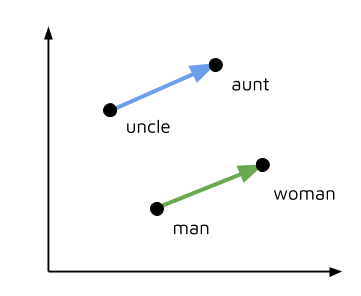
\includegraphics{Figures/word_embeddings}
\decoRule
\caption[Word vectors]{Example of collinearity between two word vectors.}
\label{fig:word_embeddings}
\end{figure}

The task of language modeling requires the transformation of words and documents into vector representation. Simple tasks like text classification could be done using naive representations like a bag of words or one hot encoding. However, these approaches would require excessive memory usage to handle large vocabulary and usually do not infer existing semantical connections between words in a language. 

Methods of \emph{word embeddings} solve both problems, providing dense vectors of real numbers, which represent word positions in $n$-dimensional space. This space represents contextual similarity of the words, thus word embeddings support semantic relations as vector operations. For example, adding vector ‘woman’ to vector ‘uncle’ and subtracting vector ‘man’ will result in vector approximately pointing to the same point as vector ‘aunt’ (see \cref{fig:word_embeddings} for example).

\section{Long-short term memory network}
Model of LSTM network is an extension of the simple recurrent network. It can store values in the hidden layer for a short or long period of time because it uses no activation function within its recurrent components. This makes it possible to backpropagate error gradient through long sequences of data without gradient vanishing or gradient exploding. This properties allow LSTM to catch long term patterns in an input sequences and make it a perfect choice for natural language modelling.

At the time step $t$ LSTM consumes a previous value of a hidden state $h^{(t-1)}$, a memory cell $c^{(t-1)}$ and an input vector $x^{(t)}$. The new value of memory cell uses gates to forget a part of the previous value and remember a new value. Input gate calculation:

\begin{equation}
i^{(t)}=\sigma(W_i\cdot[h^{(t-1)}, x^{(t)}]+b_i)
\label{lstm:input}
\end{equation} 

Forget gate:
\begin{equation}
f^{(t)} = \sigma(W_f\cdot[h^{(t-1)},x^{(t)}] + b_f)
\label{lstm:ft}
\end{equation} 

\begin{figure}[h]
\centering
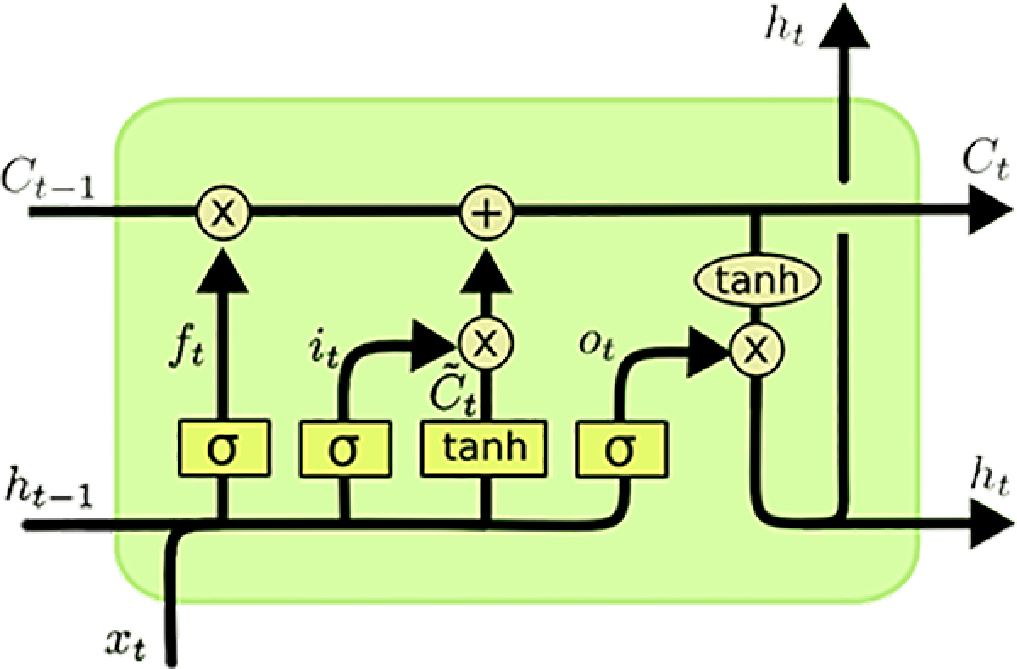
\includegraphics{Figures/lstm}
\decoRule
\caption[Long-short term memory]{Long-short term memory network achitecture \parencite{lstm-picture}.}
\label{fig:word_embeddings}
\end{figure}

New memory state:
\begin{equation}
\begin{gathered}
u^{(t)} = tanh(W_u\cdot[h^{(t-1)}, x^{(t)}]+b_u) \\

C^{(t)} = f_t\circ C^{(t-1)}+i_t\circ u^{(t)}
\end{gathered}
\label{lstm:c}
\end{equation} 

New hidden state:
\begin{equation}
\begin{gathered}
o^{(t)}=\sigma(W_o[h^{(t-1)},x^{(t)}]+b_o) \\

h^{(t)}=o^{(t)}\circ tanh(C^{(t)})
\end{gathered}
\label{lstm:h}
\end{equation} 

LSTM step can be presented as a function:
\begin{equation}
h^{(t)}, c^{(t)} = f_{lstm}(x^{(t)}, h^{(t-1)}, c^{(t-1)})
\end{equation}

The value of memory cell often is not used in a further calculations and thus can be omitted:
\begin{equation}
h^{(t)} = f_{lstm}(x^{(t)}, h^{(t-1)})
\end{equation}

For the task of natural language processing an important information about a current word can be stored not only at the previous words but also at the next words of the sentence. To catch this information a model of bidirectional LSTM (BiLSTM) was proposed  \parencite{schuster1997, graves2005}. It represents each word as a concatenation of a forward and a backward embedding:

\begin{equation}
\begin{gathered}
h_{forward}^{(t)} = f_{lstm.forward}(x^{(t)}, h^{(t-1)}_{forward}) \\
h_{backward}^{(t)} = f_{lstm.backward}(x^{(t)}, h^{(t+1)}_{backward}) \\

h^{(t)} = [h_{forward}^{(t)}, h_{backward}^{(t)} ]
\end{gathered}
\end{equation}

\section{Sequence-to-sequence machine translation} \label{seq2seq}
% http://phontron.com/class/mtandseq2seq2017/mt-spring2017.chapter8.pdf
The task of the machine translation can be formalized as a mapping of a sequence of words in a source language to a sequence of words in a target language \parencite{Neubig2017}. This task can be solved with an \emph{encoder-decoder} model, which consists of two RNNs. The first RNN consumes input sequence step by step and encodes it into so-called thought vector. After encoding, the second RNN uses thought vector as its initial hidden state and decodes an output sentence word by word.  Each word from the decoder output is used as an input for the next decoding step until the model outputs the end-of-sentence token. 

During a training, Seq2Seq model learns its parameters maximizing the log-likelihood $P(y|x)$ of the target sequence $y$ given the input sequence $x$. The next input of decoder can be selected in two ways:
    \begin{itemize}
    	\item \textbf{Without Teacher Forcing:} the previous prediction used as the next input.
    	\item \textbf{With Teacher Forcing:} A value from the target sequence used as the next input.
    \end{itemize}


\subsection{Attention} \label{attention}
Theoretically, a sufficiently large encoder-decoder model should be able to perform the machine translation perfectly. However, to encode all words and  their dependencies in the arbitrary-length sentences, the thought vector should have enormous length. Such model would require massive computational resources to train and to use,  thus this approach is ineffective.

This problem can be solved with attention technique \parencite{Bahdanau2014}. Its basic idea is to replace a single vector representation of the  input sentence with references to representations of different words in it. On the encoding step, each word representation $h_e^{(t)}$ is stored as a column of matrix $H_e$. During the decoding step, each decoder input is extended with context vector $\phi^{(t-1)}$:

\begin{equation}
h_d^{(t)} = lstm([w^{(t)}, \phi^{(t)}], h_d^{(t-1)})
\label{attn:hd}
\end{equation}

\begin{figure}
\centering
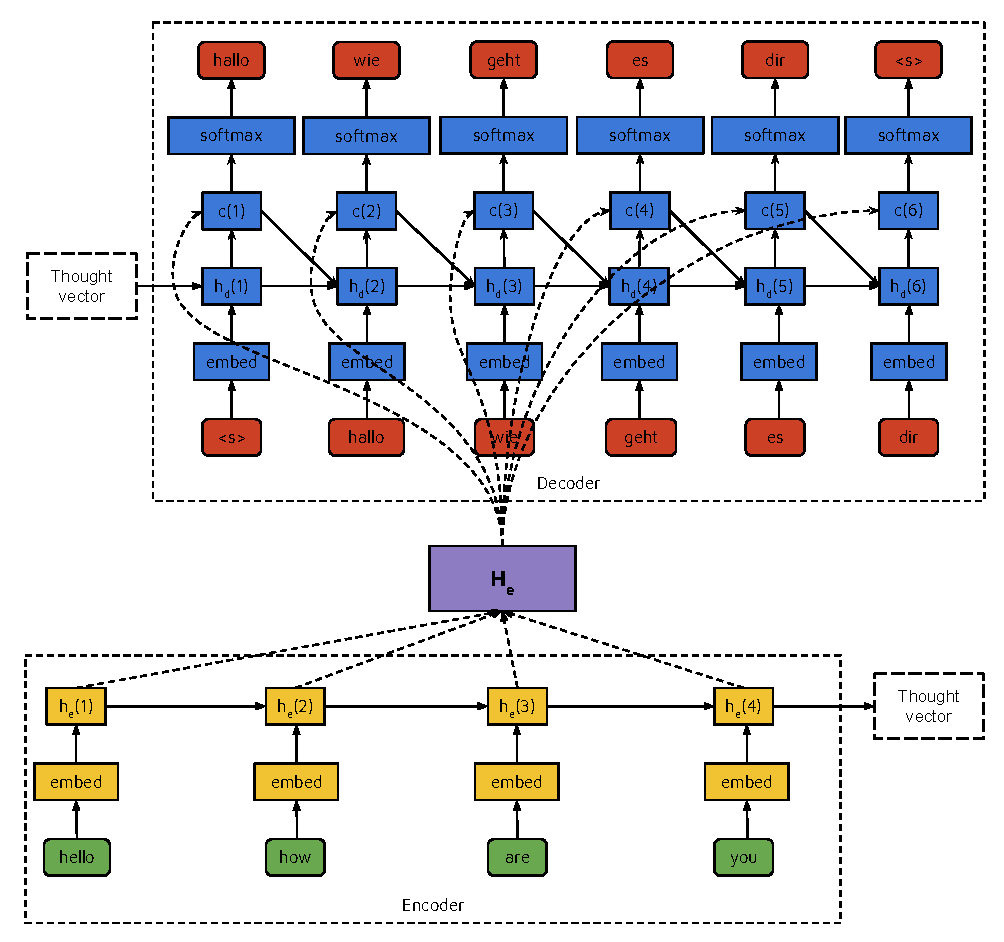
\includegraphics[width=5in]{Figures/seq2seq.pdf}
\decoRule
\caption[Seq2Seq model]{Seq2Seq with attention model.}
\label{fig:seq2seq}
\end{figure}

Context vector $\phi^{(t)}$ is calculated as a weighted sum of the encoder representations:
\begin{equation}
	\phi^{(t)} = H_e\cdot\alpha^{(t)}
	\label{attn:phi}
\end{equation}

Weights for the attention vector $\alpha^{(t-1)}$ can be calculated with an arbitrary attention score function (for example, vector product) for each pair of the decoder vector $h_d^{(t)}$ and the encoder vector $h_e^{(i)}, \forall i \in 1..n$, where $n$ is a length of the encoded sequence. In this work we used DNN with one hidden layer as suggested in the work of \cite{Bahdanau2014}:
\begin{equation}
\begin{gathered}
\hat{\alpha}_i^{(t)} = W_{attn1} \cdot [h_e^{(i)}, h_d^{(t-1)}] \\
\alpha_i^{(t)} = W_{attn2} \cdot tanh(\hat{\alpha}_{i}^{(t)}) \\
\alpha^{(t)} = softmax(\alpha^{(t)})
\end{gathered}
\label{attn:alpha}
\end{equation}

This way each decoder step can use information from an arbitrary part of encoded sequence. Input sentence representation should not be limited to fixed length thought vector, and thus it can model natural language with adequate model size. An architecture of sequence-to-sequence model with attention can be seen in \cref{fig:seq2seq}.

\subsection{Beam search} \label{beam}
When the model learned the probability model on training examples, it can generate new translations. This can be done in several ways \parencite{Neubig2017}:
        \begin{itemize}
    	\item \textbf{Random Sampling:} For each time step $t$ randomly select output words $w^{(t)}$ for $y$ from the probability distribution $P(y|x)$.
    	\item \textbf{Gready Search:} Find the $y$ that maximizes $P(y|x)$, selecting each next word $w^{(i)}$ with maximum probability $\hat{w^{(t)}} = \underset{w^{(t)}}{\operatorname{argmax}} P(w^{(i)}|x, w^{(<i)})$.
    	\item \textbf{Beam Search:} Find the $n$ outputs with the highest probabilities according to $P(y|x)$.
    \end{itemize}

\emph{Beam search} is similar to greedy search, but instead of considering only the one best hypothesis $\underset{w^{(t)}}{\operatorname{argmax}} P(w^{(i)}|x, w^{(<i)})$, it is considering $b$ best hypotheses at each time step, where $b$ is the width of the beam. To find the best hypotheses, beam search explores the generation graph in a breadth-first manner. At each level of the search tree it calculates a probability for each candidate from the target space and then selects $b$ variants with the highest probability. This way it allows to generate sequences with the higher cumulative probability, which could have been missed by the greedy search.

\section{Recursive neural networks} \label{sec:rvnn}
% reflects domain knowledge
The architecture of a recurrent neural network contains an inductive bias about a conditional probability of target variable with the previous values in a sequence. Natural language can be modeled this way, as a plain sequence of words. However, this approach ignores domain knowledge about the syntactic structure of a text. A syntactic tree contains important information about relations between individual terms and thus should not be omitted in the task of natural language modeling.

\begin{figure}[h]
\centering
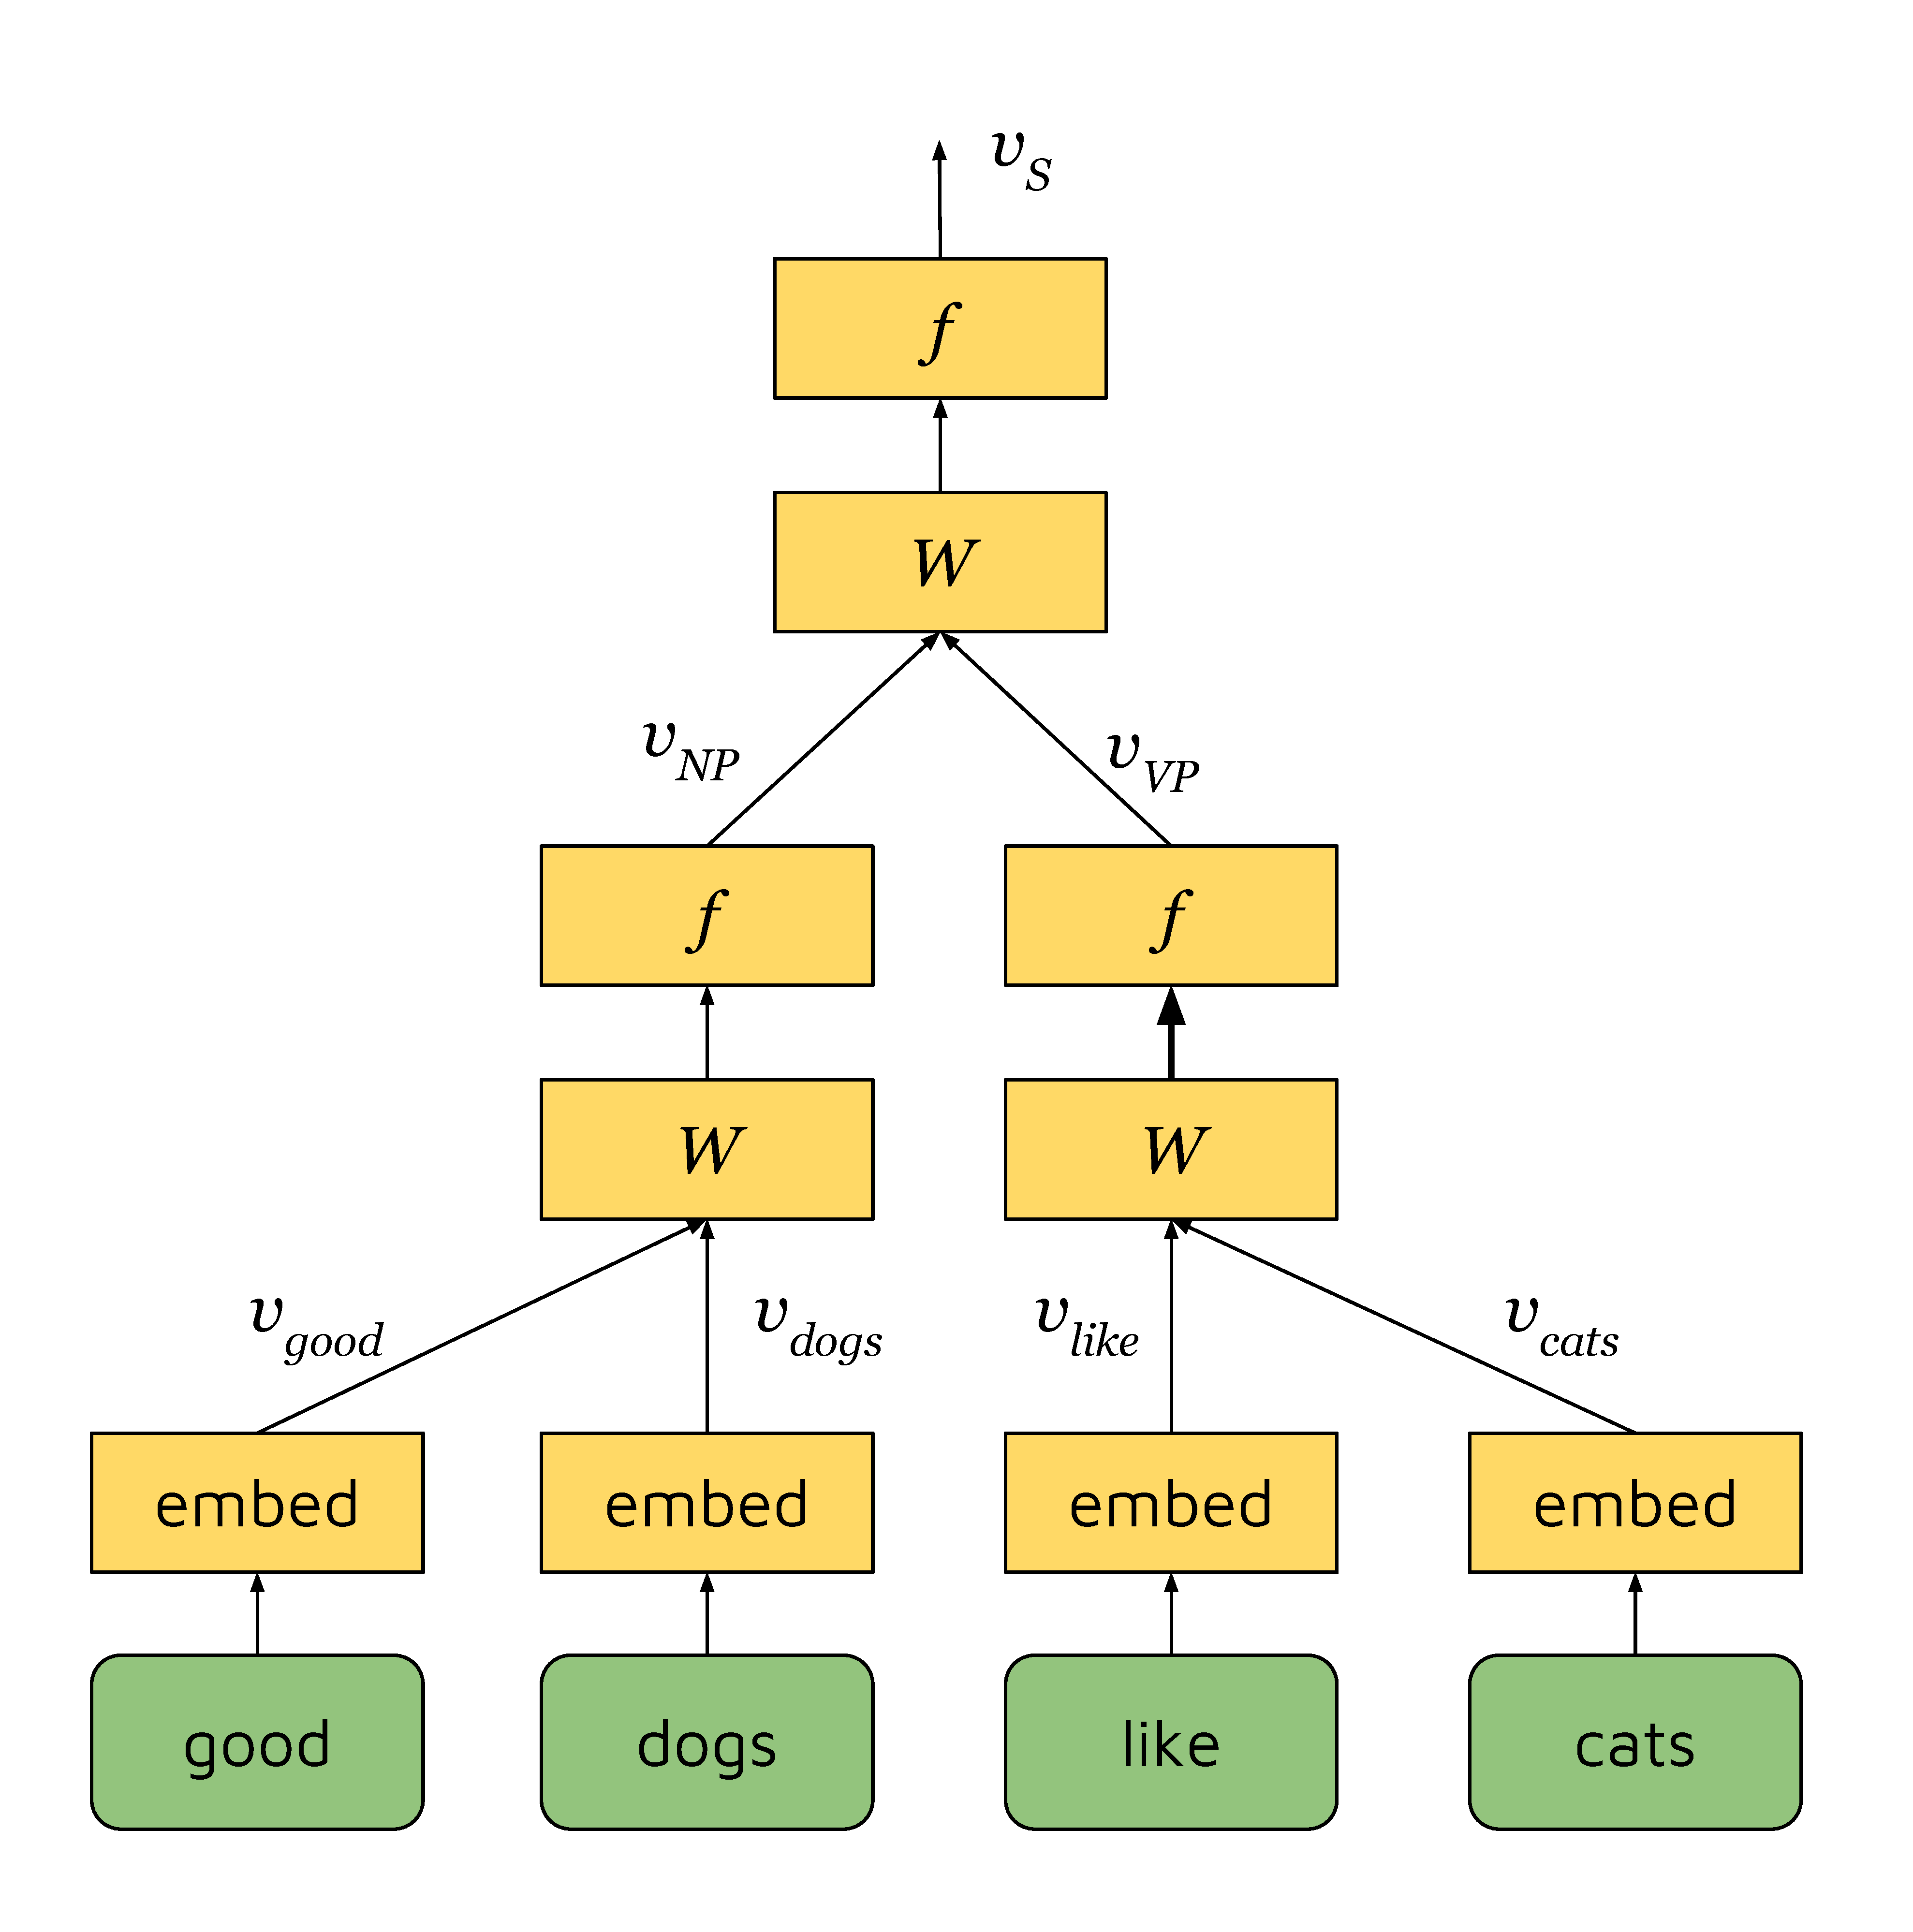
\includegraphics[width=5in]{Figures/rvnn.pdf}
\decoRule
\caption[RvNN flow]{Examle of recursive neural network flow.}
\label{fig:rvnn}
\end{figure}

Topological structures with a variable length could be modeled by neural networks recursively applying the same set of weights to each node. To model a syntactic tree, each word is represented by a corresponding embedding vector and then parent vectors are computed using a bottom-up approach with composition functions. For example, representation of the syntactic tree of the sentence \textquote{good dog like cats} could be modeled in the following way:
\begin{equation}
\begin{split}
h_{NP} = f(W\cdot[w_{good}, w_{dog}] + b)\\
h_{VP} = f(W\cdot[w_{like}, w_{cats}] + b)\\
h_S = f(W\cdot[h_{NP}, h_{VP}] + b)
\label{rvnn:example}
\end{split}
\end{equation}
where $f$ is any differentiable non-linearity like $tanh$ or $ReLU$. The example of semantic tree parsing with recursive network is presented in \cref{fig:rvnn}.

\section{Pointer networks} \label{pointer}
A neural network operates with vector representations of words that are selected from a predefined vocabulary. This imposes the problem of unknown words that don't have a vector representation. This is especially important for the translation task where both an input and an output sequences could contain rare, special words or names. However, names of people or locations should not be translated but copied to a target sequence. \cite{Vinyals2015} proposed a solution of this problem with \emph{pointer network}. For each decoding step it calculates the probability of the next word to be copied from an input sequence. Calculation of this probability is described below step-by-step.

Let's denote $H_{encoder}$ as a matrix of encoder output vectors and $h_{decoder}^{(t)}$ - decoder output vector on decoding step $t$. First a hidden state of a pointer network is calculated:

\begin{equation}
    \begin{gathered}
    
    H_{e.pointer} = H_e \cdot W_{e}\\
    
    h_{d.pointer} = h_{d}^{(t)} \cdot W_{d}\\
    
    H_{pointer} = tanh(H_{e.pointer} + h_{d.pointer})\\
    
    \end{gathered}
    \label{eq:pointer}
\end{equation}

Then each row from the matrix $H_{pointer}$ is translated to one value and probability calculated as result of $softmax$:

\begin{equation}
    \begin{gathered}
    
    H_{prob} = H_{pointer} \cdot W_{pointer}\\
    
    P = softmax(H_{prob})\\
    
    \end{gathered}
\end{equation}

Vector $P$ contains a probability for each input sequence token to be copied into the output sequence. In the following explanations, a pointer network function is denoted $f_{pointer}$:
\begin{equation}
    P = f_{pointer}(H_e, h_d^{(t)})
\end{equation}